%======================================================================
\subsubsection*{MOD-11 plan (25 Oct 2026, built on your recommendations)}\label{sec:mod11-plan}
%======================================================================

You chose this epic on 25 Oct and asked me to build it on my recommendations. The references are Fusion's
\textsc{Inspect} menu and SolidWorks' \emph{Evaluate} tab; your manufacturing is FDM (PETG, ABS), CNC and sheet metal
or laser. What is already there is reused, not built again: \code{Std\_Measure} (the pill's ruler), the Physical tab
of the right panel (\eref{UIX-12}: mass, volume, area, box, centre of mass, inertia about the centre or the origin,
principal axes), section views (\eref{MOD-16}) and the clash check (\eref{ASM-06}, another session; its distance code
measures between parts with \code{distToShape}, the wall thickness is a ray cast inside one solid, so nothing is
shared). New are four colour maps and a Mass Properties command.

\paragraph{Decisions and why.}
\begin{center}
\small
\begin{tabularx}{\linewidth}{@{}p{3.1cm}X@{}}
\toprule
Decision & Reason\\
\midrule
One engine, one view layer & \file{bruceworx\_analysis.py} computes (no GUI, tested in \code{FreeCADCmd});
  \file{bruceworx\_analysis\_gui.py} draws and holds the task panel. The numbers can be scripted (\eref{AUT-03}) and
  tested without a window.\\
Nothing saved in the file & An analysis lives while its task panel is open, like SolidWorks'. It takes well under a
  second, so it is cheaper to compute again than to keep in sync; the file stays stock FreeCAD. Fusion keeps analyses
  in the Browser: question Q1.\\
Drawn in its own nodes & The analysed shape's display triangles, copied into a separator at the end of the view's
  scene, unpickable, so a click still selects the part. \emph{As built:} drawing the copy just in front of FreeCAD's
  faces (polygon offset) still flickered against them, so while a map shows, the part's own faces are switched off
  with an invisible draw style placed after their \code{FaceStyle} node, and the map is drawn at the faces' own depth:
  the edges stay on top. Studio's program (\eref{UIX-08}, child 0 of the same node) is not touched. Links to a part
  share its nodes, so every visible instance of an analysed part is analysed too. Closing the panel puts it all back.\\
Colours by texture & Each vertex carries its value as a texture coordinate into a 1D colour texture, sampled
  \emph{nearest}: band edges are sharp per pixel, also inside a triangle, and a new threshold is only a new texture.
  Zebra stripes are a sphere-map texture (fixed function, no shader of our own).\\
Same triangles as the view & The mesh asks BRepMesh for FreeCAD's own display deflection, so the triangulation the
  view already made is reused and the overlay lies exactly on the faces. Normals and curvatures are the surface's own,
  at each vertex's $(u,v)$, not averaged facets.\\
Ribbon & \textsc{Design $\rangle$ Solid $\rangle$ Inspect}: Measure, Mass Properties, Overhang, Wall Thickness,
  Zebra; Draft, Curvature, Check Geometry, Clipping and Section Cut in the group's menu. \textsc{Surface} gets an
  Inspect group with Zebra, Curvature and Draft (surface quality is where they matter).\\
\bottomrule
\end{tabularx}
\end{center}

\paragraph{The tools.}
\begin{center}
\small
\begin{tabularx}{\linewidth}{@{}p{2.3cm}X>{\hsize=0.8\hsize}X@{}}
\toprule
Tool & How it is computed & Display and defaults\\
\midrule
Overhang (FDM) & Build direction $\mathbf b$ (+Z, an axis, or ``rest on a face'': $\mathbf b=-\mathbf n_f$). Angle of a
  down-facing surface from vertical $\varphi=\arcsin(-\mathbf n\cdot\mathbf b)$, Cura's convention: 0 a wall, 90 a
  ceiling. Support when $\varphi>\theta_c$. A face facing straight down at the lowest level is on the bed.
  & $\theta_c=45^\circ$; yellow 10$^\circ$ below it (prints, may sag); red needs support; blue on the bed. Support
  and bed areas in mm\textsuperscript{2}.\\
Draft (moulding) & Pull direction $\mathbf d$, draft $\delta=\arcsin(\mathbf n\cdot\mathbf d)$ & 1$^\circ$ required;
  green $\delta\ge1^\circ$, yellow $|\delta|<1^\circ$, red negative.\\
Wall thickness & Rays straight into the material from every vertex (nudged off the edges) and every triangle centre
  to where they leave the solid (the first face turned away from the ray; grazing hits ignored; a hit on the ray's own
  or a neighbouring face counts only where that face turns back against it, over 120$^\circ$, as a fin's other side
  does, not at a hole's mouth in a curved hub). Möller--Trumbore in
  numpy, a grid of cells as wide as the longest ray keeps the candidates near each ray. Rays end at a cap of twice the
  target: anything thicker is ``thick enough''.
  & FDM 0.4\,mm nozzle: red under 0.8\,mm (two lines: prints, weak), orange under 1.2\,mm (three lines, the usual
  minimum), green above. Presets for a 0.6\,mm nozzle and CNC (aluminium 0.5/1.0, plastics 1.0/1.5). Thinnest wall,
  where, and the area under each limit.\\
Curvature & $k_1,k_2$ from OCCT (\code{GeomLProp}) at each vertex, sign flipped on reversed faces so convex is
  positive. Mean $H=(k_1+k_2)/2$ (default), Gaussian $K=k_1k_2$, or the largest $|k|$. & Blue--green--red ramp
  over $\pm$ the 95th percentile \emph{by area} (small fillets have many vertices), so a few small fillets do not wash
  out the rest; one range for all parts; legend in 1/mm and as a radius.\\
Zebra & Reflection of a striped environment: the stripes stay with the view while the part turns. A kink in the
  stripes at an edge is a tangency (G1) break, a jump a position (G0) break. & 12 stripes, horizontal or vertical.\\
Mass properties & Already in the Physical tab. The command opens it; a fixture checks the numbers by hand (below).
  & ---\\
\bottomrule
\end{tabularx}
\end{center}

Limits I accept for now: the overhang map also marks bridges (a short flat ceiling between two walls prints without
support) and does not find islands (a lowest point in mid-air); the ray method reads a tapering feature (a gear
tooth's tip) thicker than its narrowest width, and it says nothing about walls that are too thick (sink marks in
moulding). Section planes (\eref{MOD-16}) do not cut the overlay.

\paragraph{Performance budget.} Spike on 25 Oct in \code{FreeCADCmd} (FreeCAD 1.1.4, numpy 1.26), housing
\code{LE-01-01003} (297 faces, 12\,064 triangles) and planet gear \code{LE-01-01008} (183 faces, 8\,136):
the mesh with normals 0.17\,s and 0.11\,s (first try 7.9\,s: \code{Face.valueAt}/\code{normalAt} build an adaptor
per call; the face's \code{Surface} is a thousand times faster), overhang 2\,ms, thickness 0.48\,s and 0.66\,s.
Budget: a map under 1\,s on a 20\,000-triangle part, a threshold or direction change under 0.1\,s, the panel's first
paint under 1.5\,s.

\paragraph{Mass properties fixture and a fix.} A steel (\code{Steel-1C45}, 7\,800\,kg/m\textsuperscript{3}) block
$40\times20\times10$\,mm with a $\varnothing10\times20$\,mm cylinder standing on it at $(30,10)$: hand values for
mass, centre and the inertia tensor, compared with the Physical tab's numbers to $10^{-6}$. On the way:
\code{partprops.computed\_mass} read the density with \code{getPhysicalValue}, which in FreeCAD~1.1 writes the material
back and touches the body (checked: \code{Up-to-date} before, \code{Touched} after, on \code{LE-01-01009}). It now
reads the material's \code{PhysicalProperties}; a regression test keeps it that way.

\paragraph{Acceptance (proposed).} (1) The fixture's mass, CG and inertia match the hand calculation. (2) Overhang
fixtures: a cantilever's 200\,mm\textsuperscript{2} underside and the upper quarter of a horizontal $\varnothing10$
hole ($\pi r L/2=157.1$\,mm\textsuperscript{2}) flagged within 2\,\%; a 2\,mm plate reads 2.00\,mm thick, a
0.6\,mm one too thin. (3) On a copy of the gearbox: the housing's overhang map printed flange-down and upside down,
the planet gear's thin tooth tips, zebra on the carrier; studio still on, the file not modified, a click still
selects the part, closing the panel leaves the scene as it was.

\paragraph{Built 25 Oct.} Five commits: the engine (\file{bruceworx\_analysis.py}, 20 fixture tests in
\code{TestBruceWorxAnalysis}), the view layer and panel (\file{bruceworx\_analysis\_gui.py}, GUI test
\code{TestBruceWorxInspect}), assemblies and the edge rule, and the band edges. The Physical tab's collector had a bug
found on the way: in an assembly every part is pointed at by a joint, and the filter meant for a Part Cut's operands
dropped them all, so a whole assembly showed nothing; only shape features count as results now (test). The ribbon:
\textsc{Solid $\rangle$ Inspect} reads Measure, Mass Properties, Interference, Overhang, Wall Thickness, Zebra
(Draft, Curvature, Check Geometry, Clipping, Section Cut in its menu); \textsc{Surface $\rangle$ Inspect} reads Zebra,
Curvature, Draft.

\begin{center}
\small
\begin{tabularx}{\linewidth}{@{}>{\hsize=0.8\hsize}X>{\hsize=1.2\hsize}X@{}}
\toprule
Check & Result (25 Oct, test FreeCAD on a copy of the gearbox)\\
\midrule
Mass fixture & Mass, centre and inertia tensor equal the hand values to $10^{-6}$; reading the mass leaves the part
  \code{Up-to-date}.\\
Overhang fixtures & Cantilever 200.0\,mm\textsuperscript{2} and bed 100.0; upside down, bed 300 and no support;
  horizontal $\varnothing10$ hole within 2\,\% of 157.1\,mm\textsuperscript{2}; a 45$^\circ$ chamfer needs support at a
  40$^\circ$ threshold, not at 50$^\circ$.\\
Housing \code{LE-01-01003} & Flange down (+Z): no support, 15.6\,cm\textsuperscript{2} on the bed. Upside down:
  2.2\,cm\textsuperscript{2} of support on 1 face. On its side (+X): 34.8\,cm\textsuperscript{2} on 93 faces. Thinnest
  wall 0.89\,mm (ring-gear tooth tips), 3.2\,cm\textsuperscript{2} under 1.2\,mm, none under 0.8.\\
Planet \code{LE-01-01008} & Thinnest 0.99\,mm at the tooth tips (orange, figure); smallest radius 0.38\,mm.\\
Sun \code{LE-01-01009} & \textbf{A real thin wall:} the M3 set-screw hole (\o2.5 tap drill) is 0.5\,mm from the hub's
  end face, 9.6\,mm\textsuperscript{2} under 0.8\,mm (figure). Fine in steel; for a printed sun move the hole up or
  lengthen the hub.\\
Whole gearbox \code{LE-02-01002} & 24 parts, opens in 1.05\,s; thickness map 1.9\,s; every part's faces back after
  closing; studio on 49 parts before, during and after; no document marked modified; undo stack untouched.\\
Panel & First map 0.6\,s (housing), a setting change 0.5\,s; a click through the map selects the part
  (\code{Body.Hole.Face1}); Mass Properties brings the Physical tab forward.\\
\bottomrule
\end{tabularx}
\end{center}

\begin{figure}[htbp]
\centering
\begin{subfigure}[b]{0.32\linewidth}\centering
  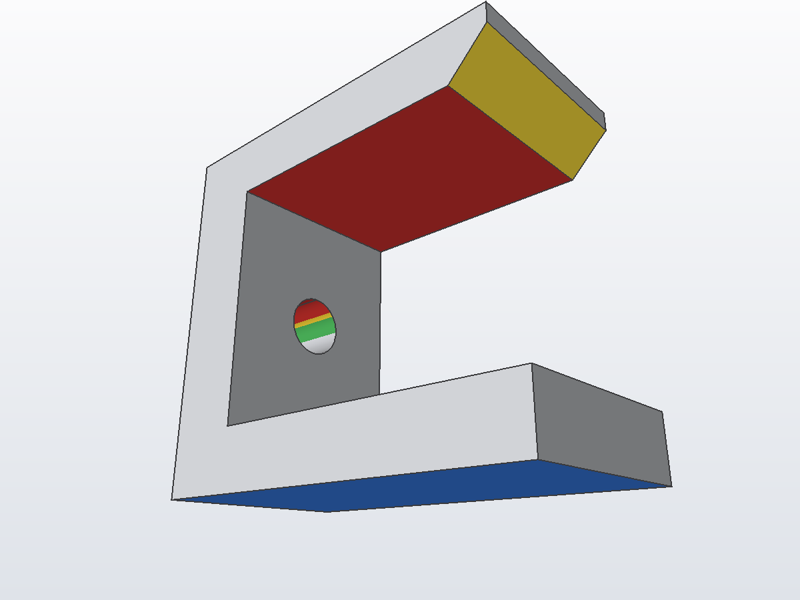
\includegraphics[width=\linewidth]{fig/mod11_bracket_overhang.png}
  \caption{Overhang, +Z: the arm's underside red, its 45$^\circ$ chamfer yellow, the hole banded, the bed blue.}
\end{subfigure}\hfill
\begin{subfigure}[b]{0.32\linewidth}\centering
  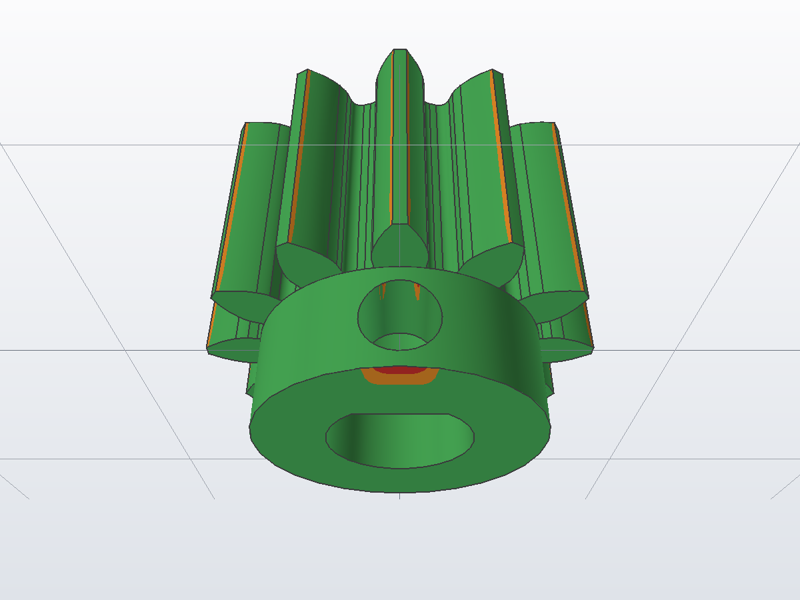
\includegraphics[width=\linewidth]{fig/mod11_sun_thickness.png}
  \caption{Sun gear: 0.5\,mm under the set-screw hole (red), the tooth tips thin (orange).}
\end{subfigure}\hfill
\begin{subfigure}[b]{0.32\linewidth}\centering
  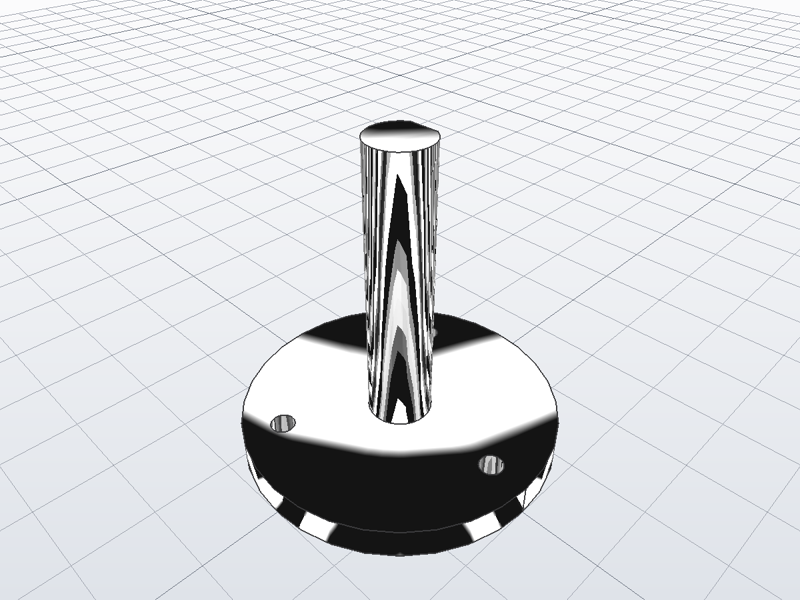
\includegraphics[width=\linewidth]{fig/mod11_carrier_zebra.png}
  \caption{Zebra on the carrier: the stripes run on smoothly over the shaft.}
\end{subfigure}
\caption{Inspect maps in the test FreeCAD, 25 Oct (saved images of the 3D view; studio shading on for the other
parts). (a) is a test bracket, (b) and (c) are copies of the gearbox's sun gear and carrier.}
\label{fig:mod11-maps}
\end{figure}

What to try by hand: select the housing, \textsc{Inspect $\rangle$ Overhang}, set the build direction to $-$Z or pick
\emph{Selected face} with the flange selected; \textsc{Wall Thickness} on the sun gear and turn it to see the red patch
under the set screw; \textsc{Zebra} on the carrier while orbiting; nothing selected analyses every visible part.

\paragraph{Questions.}
\begin{enumerate}[nosep,label=Q\arabic*]
\item Keep analyses in the file, in the Browser with an eye, as Fusion does? (Now: they live while the panel is open.)
\item Are 0.8 and 1.2\,mm the right wall limits for your PETG/ABS prints (0.4\,mm nozzle)?
\item Should the build direction be a part property (\eref{MFG-01}'s print orientation) that the overhang map reads
  and writes?
\item Mark short flat ceilings as bridges (for example up to 10\,mm) rather than as needing support?
\item Sheet metal and laser: anything to inspect beyond \eref{MOD-06}'s rules (minimum hole or slot against the
  thickness, minimum flange)?
\item In an assembly each part is judged as printed on its own (its own bed) but in the assembly's orientation. Keep
  that, or use each part file's own orientation?
\item \file{bruceworx\_board.py} (\eref{ECD-06}) still reads the density with \code{getPhysicalValue}, which touches
  the body; it belongs to another epic, so I left it. Fix it the same way?
\end{enumerate}
